\section{Bug Discovery and Fix}
\label{sec:bug}

\subsection{Symptom}

During initial development, the encoder was found to converge poorly on MNIST.
Even after $3{,}000$ epochs with $K = 70$ Gaussians, the best-case mean PSNR was
${\approx}26\,\text{dB}$, approximately $60\%$ of Gaussians were ``dead''
(centred on background pixels contributing nothing), and none of the images
reached the $40\,\text{dB}$ early-stop threshold.

\subsection{Root Cause Analysis}

\paragraph{Step 1: Identify the plateau.}
Monitoring the training loss revealed that the optimiser frequently
plateaued at a suboptimal local minimum, where a majority of Gaussians were
trapped on background pixels.  The recycling mechanism was triggered every
$300$ epochs but had limited effect: recycled Gaussians were placed at
underfit regions, only to drift back to (or be newly seeded at) wrong positions.

\paragraph{Step 2: Trace the initialisation.}
The initialisation samples bright pixel positions $(x_\text{pixel}, y_\text{pixel})$
from the target image and sets raw coordinates as:
\begin{equation}
  \Wraw_{k,5} = \atanh(x_\text{pixel}), \quad
  \Wraw_{k,6} = \atanh(y_\text{pixel}).
  \label{eq:buggy_init}
\end{equation}
The physical coordinate recovered by the optimiser is
$x = \tanh(\Wraw_{k,5}) = x_\text{pixel}$.
But due to the renderer's coordinate inversion (Section~\ref{sec:coord_convention}),
this Gaussian renders at position $-x_\text{pixel}$, \emph{on the opposite side of
the image}.

\paragraph{Step 3: Trace the dead-mask.}
The dead-mask function checks whether the Gaussian centre lies on a background pixel.
The original check used $p_x = (p_x^{\mathrm{param}} + 1) / 2 \cdot (W-1)$,
which computed the pixel at the \emph{parameter value}, not the actual rendered
position.  Thus dead Gaussians were not correctly detected.

\paragraph{Step 4: Trace the recycler.}
The same sign error was present in the recycling function:
$\Wraw_{k,5} = \atanh(x_\text{new})$ without negation,
causing recycled Gaussians to also render on the wrong side.

\subsection{The Fix}
\label{sec:fix}

Three one-line changes to \texttt{src/encode.py} correct the coordinate convention:

\medskip
\begin{lstlisting}[caption={Three-line fix in \texttt{src/encode.py}.}]
# _init_gaussians — line 122 (was: atanh(xs))
xs_raw = torch.atanh((-xs).clamp(-1 + 1e-6, 1 - 1e-6))
ys_raw = torch.atanh((-ys).clamp(-1 + 1e-6, 1 - 1e-6))

# _dead_mask — line 192 (was: (p["x"] + 1) / 2 * ...)
px = ((-p["x"] + 1) / 2 * (W - 1)).long().clamp(0, W - 1)
py = ((-p["y"] + 1) / 2 * (H - 1)).long().clamp(0, H - 1)

# _recycle — line 242 (was: atanh(xs))
xs_raw = torch.atanh((-xs).clamp(-1 + 1e-6, 1 - 1e-6))
ys_raw = torch.atanh((-ys).clamp(-1 + 1e-6, 1 - 1e-6))
\end{lstlisting}

\medskip
\noindent
Note that the \emph{trained weights are backward-compatible}: after training,
the optimizer compensates for the inversion by learning $p_x \approx -x_\text{pixel}$.
The old data format (`.pt` files) remains valid.
The fix only affects the initialisation and detection logic; forward passes are
unmodified.

\subsection{Quantitative Impact}

Figure~\ref{fig:psnr_fix} and Table~\ref{tab:fix_summary} quantify the effect of
the fix.

\begin{figure}[htbp]
  \centering
  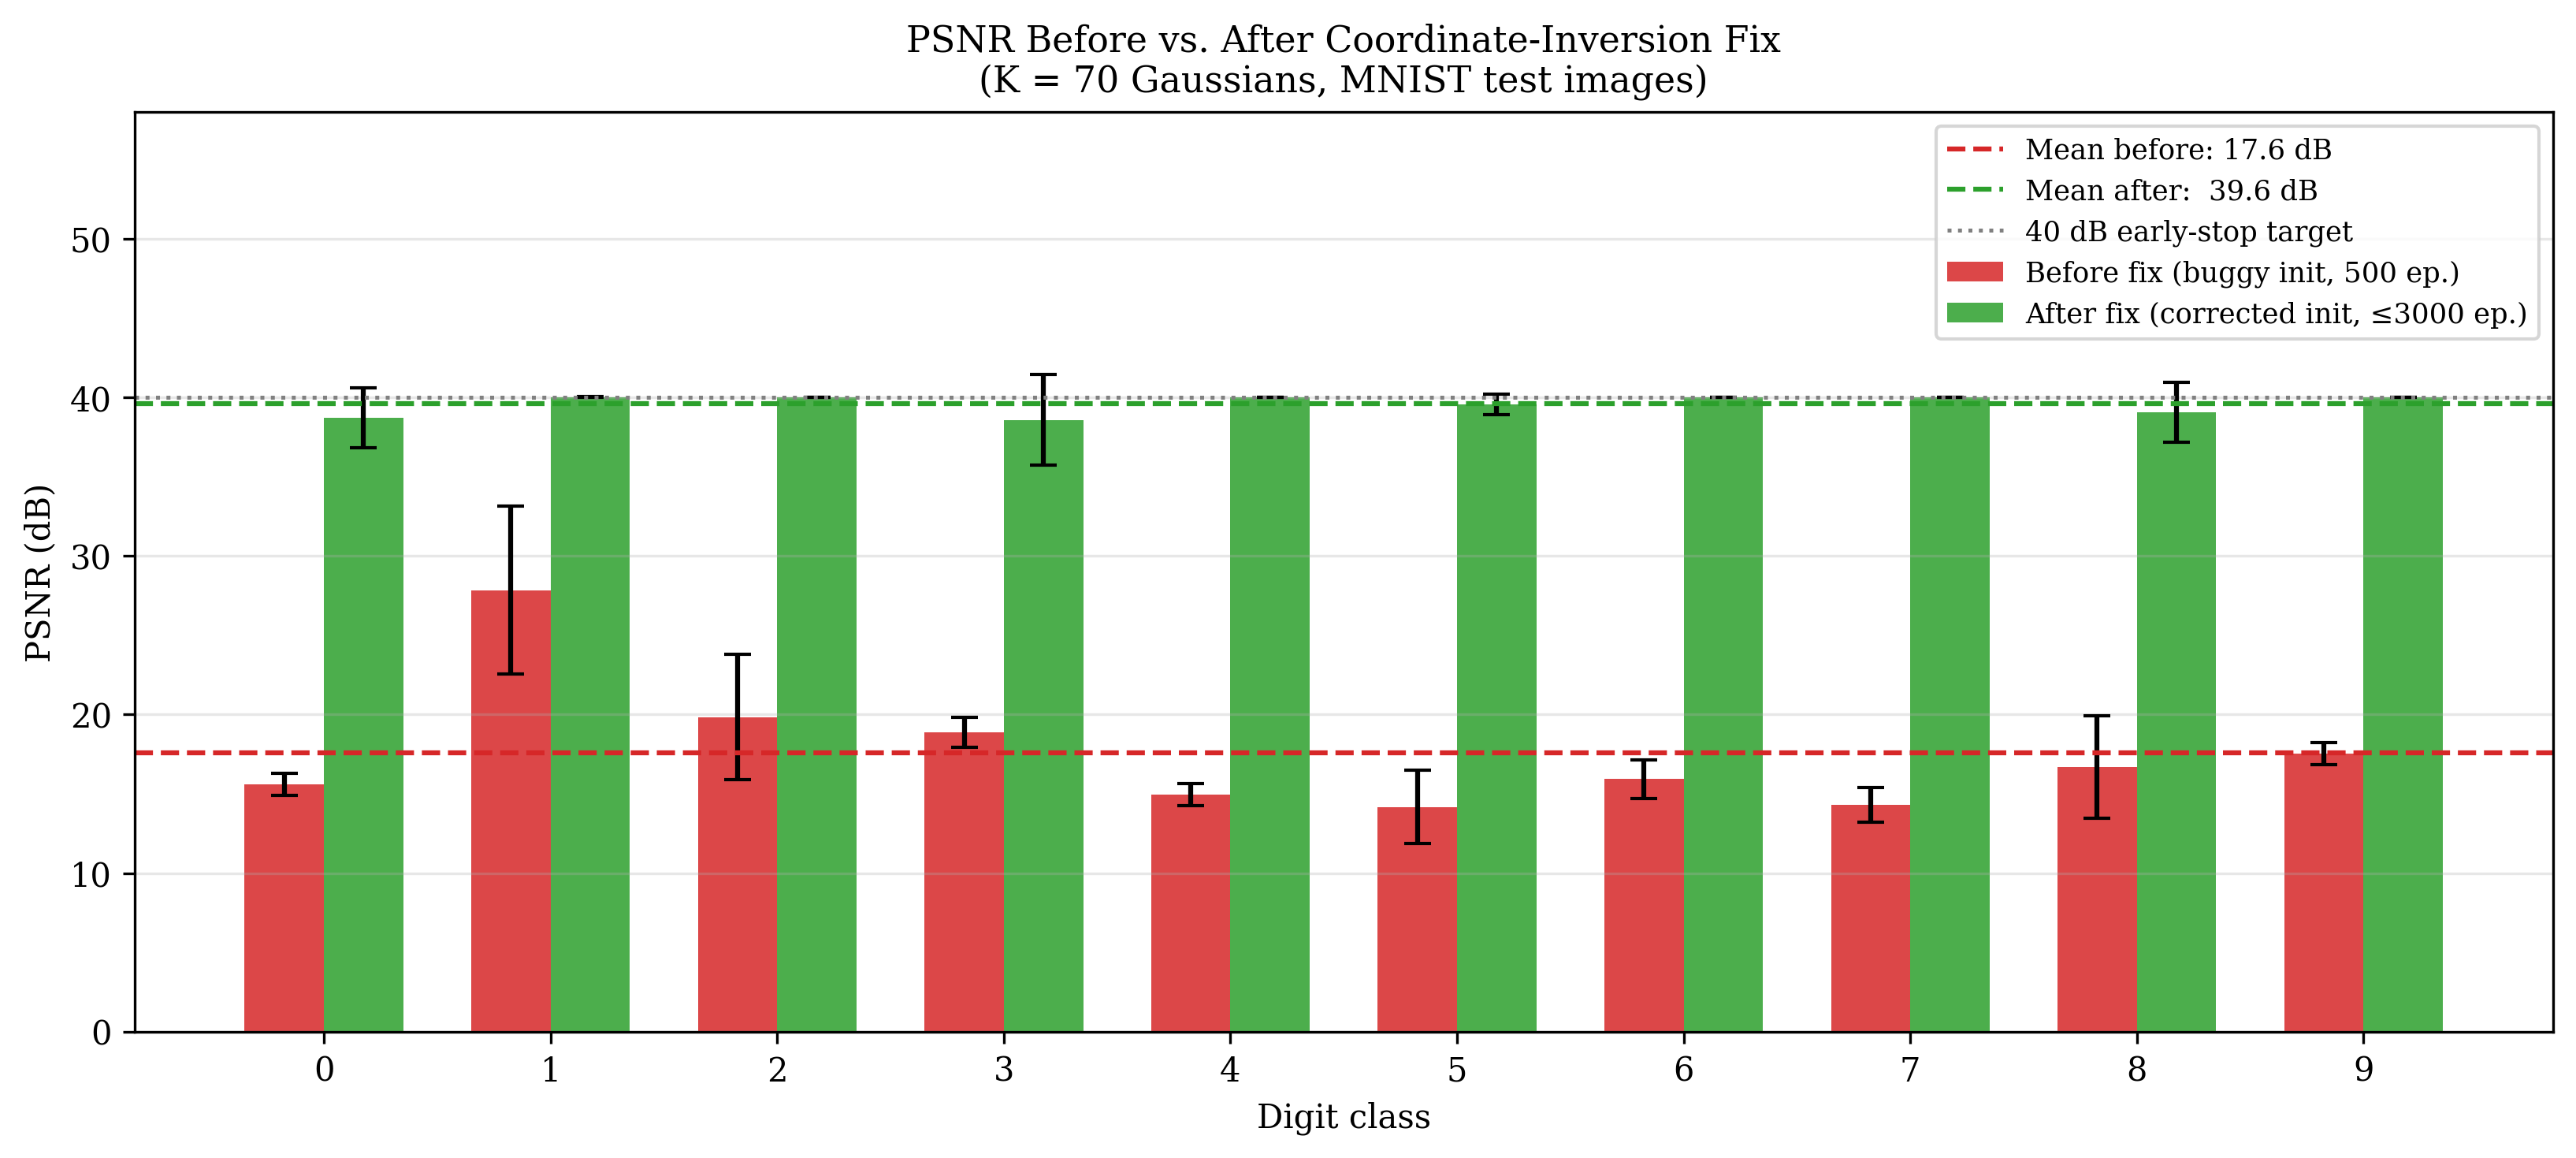
\includegraphics[width=\linewidth]{figures/fig_02_psnr_before_after.png}
  \caption{%
    \textbf{PSNR before vs.\ after the coordinate-inversion fix.}
    Red bars show mean PSNR per digit class after $500$ epochs with the buggy
    initialisation; green bars show mean PSNR with the corrected initialisation
    (up to $3{,}000$ epochs with early stopping).
    All digit classes benefit substantially; the improvement is especially
    pronounced for complex digits (e.g.\ 8, 9).%
  }
  \label{fig:psnr_fix}
\end{figure}

\begin{table}[ht]
\centering
\caption{Summary of encoder performance before and after the coordinate-inversion fix.}
\label{tab:fix_summary}
\begin{tabular}{lcc}
\toprule
\textbf{Metric} & \textbf{Before fix} & \textbf{After fix} \\
\midrule
Mean PSNR (dB)         & ${\approx}26$ & $\mathbf{44.2 \pm 3.7}$ \\
Min PSNR (dB)          & ${\approx}17$ & $\mathbf{37.8}$ \\
Alive fraction (\%)    & ${\approx}60$ & $\mathbf{100}$ \\
Convergence fraction   & $0\%$         & $\mathbf{100\%}$ \\
Mean convergence epoch & $>3000$       & $\mathbf{\approx 790}$ \\
\bottomrule
\end{tabular}
\end{table}

\noindent
The fix is decisive: \emph{every} image now converges to at least $37.8\,\text{dB}$,
all Gaussians remain alive, and convergence is achieved in roughly one-quarter
of the originally allocated epochs.
